\documentclass[17pt]{beamer} %Makes presentation
%\documentclass[handout, 17pt]{beamer} %Makes Handouts
\documentclass[17pt]{beamer} %Makes presentation
%\documentclass[handout]{beamer} %Makes Handouts
\usetheme{Singapore} %Gray with fade at top
\useoutertheme[subsection=false]{miniframes} %Supppress subsection in header
\useinnertheme{rectangles} %Itemize/Enumerate boxes
\usecolortheme{seagull} %Color theme
\usecolortheme{rose} %Inner color theme

\definecolor{light-gray}{gray}{0.75}
\definecolor{dark-gray}{gray}{0.55}
\setbeamercolor{item}{fg=light-gray}
\setbeamercolor{enumerate item}{fg=dark-gray}

\setbeamertemplate{navigation symbols}{}
%\setbeamertemplate{mini frames}[default]
%\setbeamercovered{dynamics}
\setbeamerfont*{title}{size=\Large,series=\bfseries}
\setbeamerfont{footnote}{size=\tiny}

%\setbeameroption{notes on second screen} %Dual-Screen Notes
%\setbeameroption{show only notes} %Notes Output

\setbeamertemplate{frametitle}{\vspace{.5em}\bfseries\insertframetitle}
\newcommand{\heading}[1]{\noindent \textbf{#1}\\ \vspace{1em}}

\usepackage{bbding,color,multirow,times,ccaption,tabularx,graphicx,verbatim,booktabs}
\usepackage{colortbl} %Table overlays
\usepackage[english]{babel}
%\usepackage[latin1]{inputenc}
%\usepackage[T1]{fontenc}
\usepackage{lmodern}

%\author[]{Thomas J. Leeper}
\institute[]{
  \inst{}%
  Department of Government\\London School of Economics and Political Science
}

\usepackage{tikz}
\usetikzlibrary{shapes,arrows,decorations.pathreplacing,calc}

\newcounter{itemnum}

\newcommand{\nt}[2][0pt]{%
    \stepcounter{itemnum}%
    \if###2##%
    \else
        #2%
        \thinspace
    \fi
    \tikz[overlay,remember picture,baseline=(\theitemnum.base),xshift=#1]\node (\theitemnum){};%
}

\newcommand{\makebrace}[4][0pt]{%
    \begin{tikzpicture}[overlay, remember picture]
        \draw [decoration={brace,amplitude=0.5em},decorate]
        let \p1=(#2), \p2=(#3) in
        ({max(\x1+#1,\x2+#1)}, {\y1+1.75ex}) -- 
            node[right=0.6em] {#4} ({max(\x1+#1,\x2+#1)}, {\y2-0.5ex});
    \end{tikzpicture}%
}

\newenvironment{braceitems}{%
    \begin{enumerate}
}{%
    \end{enumerate}
    \setcounter{itemnum}{0}%
}


\title{Tabulation and Visualization}

\date[]{}

\begin{document}

\frame{\titlepage}

\frame{\tableofcontents}



\frame{
\frametitle{Preview: Analysis}

Analysis is the ``systematic and detailed examination of data.''

\vspace{1em}

Two broad categories of analytic strategies:

\begin{enumerate}
\item Quantitative analysis
\item Qualitative analysis
\end{enumerate}


}

\frame{
\frametitle{Preview: Quantitative Analysis}

\begin{itemize}\itemsep0.5em
\item \textit{Quantitative analysis} involves calculation of statistic(s)
	\begin{itemize}
	\item Statistic: ``a quantitative summary of a variable for a set of units''
	\end{itemize}
\item<2-> Examples
	\begin{itemize}
	\item Total: Count, sum, proportion
	\item Centrality: Mean, median, mode
	\item Dispersion: Variance, standard deviation
	\item Relationship: Correlation, etc.
	\end{itemize}
\end{itemize}

}

\frame{
\frametitle{Preview: Qualitative Analysis}

\begin{itemize}\itemsep0.5em
\item \textit{Qualitative analysis} involves typically narrative characterisations of phenomena
\item<2-> Examples
	\begin{itemize}
	\item Typologies
	\item Hierarchies
	\item Accounts or interpretations
	\end{itemize}
\item<3-> \textit{Qualitative analysis} is more general and fluidic than quantitative
\end{itemize}

}





\section{Getting a grip on data}
\frame{\tableofcontents[currentsection]}


\frame{

\frametitle{Types of Measures}

\begin{braceitems}\itemsep1em
\item \nt{Categorical}
	\begin{itemize}
	\item Binary
	\end{itemize}
\item \nt{Ordinal}
\item \nt{Interval}
\end{braceitems}
\makebrace{1}{2}{Qualitative}
\makebrace{2}{3}{Quantitative}

\vspace{0.5em}

{\small Note: \textit{Ratio} scale measures are interval measures with a non-arbitrary zero value}

}



\frame{
\frametitle{Definitions}
\begin{itemize}\itemsep1.5em
\item Statistic: ``a quantitative summary of a variable for a set of units''
\item Three parts:
	\begin{itemize}
	\item A set of units
	\item A variable measured for those units
	\item An estimator (i.e., aggregation procedure)
	\end{itemize}
\end{itemize}
}

% library("gapminder")
% x <- gapminder[gapminder$year == 2007, c("country", "continent", "lifeExp", "pop"),]
% set.seed(123)
% (z <- x[sample.int(nrow(x), 10),])


\begin{frame}[fragile]
\footnotesize
\begin{verbatim}
            country continent lifeExp      pop
            Austria    Europe     79   8199783
  Equatorial Guinea    Africa     51    551201
            Iceland    Europe     81    301931
               Iran      Asia     70  69453570
             Kuwait      Asia     77   2505559
            Lesotho    Africa     42   2012649
             Serbia    Europe     74  10150265
              Sudan    Africa     58  42292929
             Sweden    Europe     80   9031088
Trinidad and Tobago  Americas     69   1056608
\end{verbatim}
\end{frame}

% central tendency

\frame<1-2>[label=centraltendency]{
\frametitle{Central Tendency}

\begin{itemize}\itemsep1.5em
\item<2-> Mean (average): $\bar{x} = \frac{1}{n}\sum\limits_{i=1}^{n} x_i$
\item<3-> Sort-based statistics:
	\begin{itemize}
	\item Range
	\item Minimum
	\item Median (middle value)
	\item Maximum
	\item Percentiles
	\end{itemize}
\item<4-> Mode: Most common value
\end{itemize}

}

\begin{frame}[fragile]
\frametitle{{\normalsize Mean/average}}
\footnotesize
\begin{verbatim}
            country continent lifeExp      pop
            Austria    Europe     79   8199783
  Equatorial Guinea    Africa     51    551201
            Iceland    Europe     81    301931
               Iran      Asia     70  69453570
             Kuwait      Asia     77   2505559
            Lesotho    Africa     42   2012649
             Serbia    Europe     74  10150265
              Sudan    Africa     58  42292929
             Sweden    Europe     80   9031088
Trinidad and Tobago  Americas     69   1056608
\end{verbatim}

\vspace{-1.5em}
\begin{align*}
Sum &= 79 + 51 + 81 + 70 + 77 + 42 + 74 + 58 + 80 + 69 = 681\\
Mean &= 681/10 = 68.1\\
\end{align*}

\end{frame}


\againframe<2-3>{centraltendency}

\begin{frame}[fragile]
\frametitle{\normalsize{Median, Min, Max, etc.}}
\footnotesize
\begin{verbatim}
            country continent lifeExp      pop
            Austria    Europe     79   8199783
  Equatorial Guinea    Africa     51    551201
            Iceland    Europe     81    301931
               Iran      Asia     70  69453570
             Kuwait      Asia     77   2505559
            Lesotho    Africa     42   2012649
             Serbia    Europe     74  10150265
              Sudan    Africa     58  42292929
             Sweden    Europe     80   9031088
Trinidad and Tobago  Americas     69   1056608
\end{verbatim}
\end{frame}

\begin{frame}[fragile]
\frametitle{Median, Min, Max, etc.}
\footnotesize
\begin{verbatim}
            country continent lifeExp      pop
            Lesotho    Africa     42   2012649
  Equatorial Guinea    Africa     51    551201
              Sudan    Africa     58  42292929
Trinidad and Tobago  Americas     69   1056608
               Iran      Asia     70  69453570
             Serbia    Europe     74  10150265
             Kuwait      Asia     77   2505559
            Austria    Europe     79   8199783
             Sweden    Europe     80   9031088
            Iceland    Europe     81    301931
\end{verbatim}
\end{frame}


\againframe<3-4>{centraltendency}

\begin{frame}[fragile]
\frametitle{Mode}
\footnotesize
\begin{verbatim}
            country continent lifeExp      pop
            Austria    Europe     79   8199783
  Equatorial Guinea    Africa     51    551201
            Iceland    Europe     81    301931
               Iran      Asia     70  69453570
             Kuwait      Asia     77   2505559
            Lesotho    Africa     42   2012649
             Serbia    Europe     74  10150265
              Sudan    Africa     58  42292929
             Sweden    Europe     80   9031088
Trinidad and Tobago  Americas     69   1056608
\end{verbatim}
\end{frame}

\begin{frame}[fragile]
\frametitle{Mode}
\footnotesize
\begin{verbatim}
            country continent lifeExp      pop
  Equatorial Guinea    Africa     51    551201
            Lesotho    Africa     42   2012649
              Sudan    Africa     58  42292929
Trinidad and Tobago  Americas     69   1056608
               Iran      Asia     70  69453570
             Kuwait      Asia     77   2505559
            Austria    Europe     79   8199783
            Iceland    Europe     81    301931
             Serbia    Europe     74  10150265
             Sweden    Europe     80   9031088
\end{verbatim}
\end{frame}

\againframe<4->{centraltendency}

\frame{
\frametitle{Dispersion/variation}

\begin{itemize}\itemsep1.5em
\item Variance:\\
	$Var(x) = s_x^2 = \sum\limits_{i=1}^{n} \frac{(x_i - \bar{x})^2}{n-1}$

\item<2-> Standard Deviation:\\ 
	$sd(x) = s_x = \sqrt{Var(x)}$
\end{itemize}

}

\begin{frame}[fragile]
\footnotesize
\begin{verbatim}
            country continent lifeExp      pop
            Austria    Europe     79   8199783
  Equatorial Guinea    Africa     51    551201
            Iceland    Europe     81    301931
               Iran      Asia     70  69453570
             Kuwait      Asia     77   2505559
            Lesotho    Africa     42   2012649
             Serbia    Europe     74  10150265
              Sudan    Africa     58  42292929
             Sweden    Europe     80   9031088
Trinidad and Tobago  Americas     69   1056608
\end{verbatim}

\vspace{-1.5em}
\begin{align*}
Mean &= 68.1\\
Variance &= \sum\limits_{i=1}^{n} \frac{(x_i - \bar{x})^2}{n-1} &= \dfrac{1620.9}{10-1} &= 180.1 \\
SD &= \sqrt{Var(x)} & &= 13.42 \\
\end{align*}


\end{frame}


\frame{
\frametitle{Shape}

\begin{itemize}\itemsep1em
\item Skewness
	\begin{itemize}
	\item<2-> Positive/right skew
	\item<2-> Symmetric
	\item<2-> Negative/left skew
	\end{itemize}
\item<3-> Kurtosis: peakedness of a distribution
\end{itemize}

}

% 

\frame{
\frametitle{Skewness}
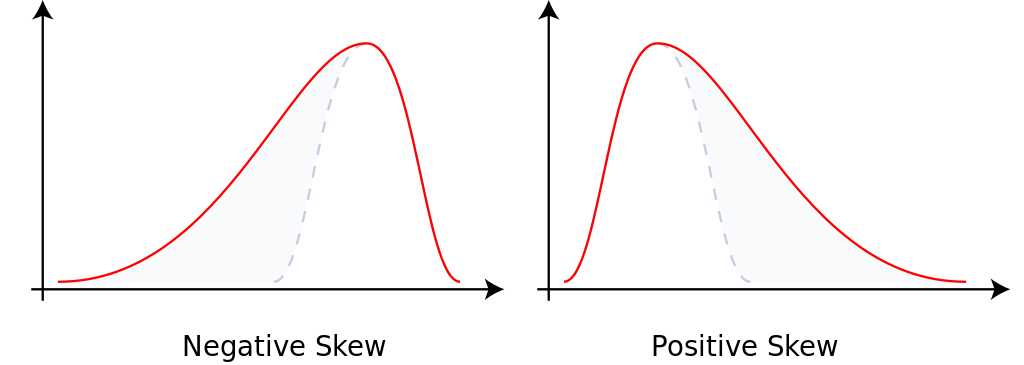
\includegraphics[width=\textwidth]{images/skew.png}
\vspace{2em}
{\tiny Source: \href{https://commons.wikimedia.org/wiki/File:Negative_and_positive_skew_diagrams_(English).svg}{Rodolfo Hermans (Wikimedia)}}
}

% relationship with other variables

\frame{
\frametitle{Relationship}

\begin{itemize}\itemsep2em
\item<1-> Covariation:\\
	$Cov(x,y) = \sum_{i=1}^{n} \frac{(x_i - \bar{x})(y_i - \bar{y})}{n-1}$
\item<2-> Correlation:\\
	{\small $Corr(x,y) = r_{x,y} = \sum\limits_{i=1}^{n} \frac{(x_i - \bar{x})(y_i - \bar{y})}{(n-1)s_x s_y}$}
\end{itemize}
}

% ggplot(z, aes(x = pop, y = lifeExp, colour = continent)) + geom_point(size = 3) + theme_bw() + theme(legend.position = c(0.9,0.2)) + geom_hline(yintercept = mean(z$lifeExp)) + geom_vline(xintercept = mean(z$pop))


\frame{
\begin{center}
\includegraphics[height=.9\textheight]{images/gapminder-mini.png}
\end{center}
}


\frame{
\frametitle{In R\dots}

\small

\begin{itemize}
\item \texttt{mean()}
\item \texttt{median()}, \texttt{min()}, \texttt{max()}, \texttt{quantile()}
\item \texttt{var()}
\item \texttt{sd()}
\item \texttt{cov()}
\item \texttt{cor()}
\end{itemize}

}

\section{Tabulation}
\frame{\tableofcontents[currentsection]}

\frame{
\frametitle{Table}
\begin{itemize}\itemsep1em
\item Definition: ``an arrangement of information into rows and columns''
\item Tables can show:
	\begin{itemize}
	\item Values
	\item Counts
	\item Proportions
	\item Summary statistics
	\end{itemize}
\end{itemize}

}

\begin{frame}[fragile]
\footnotesize
\begin{verbatim}
            country continent lifeExp      pop
            Austria    Europe     79   8199783
  Equatorial Guinea    Africa     51    551201
            Iceland    Europe     81    301931
               Iran      Asia     70  69453570
             Kuwait      Asia     77   2505559
            Lesotho    Africa     42   2012649
             Serbia    Europe     74  10150265
              Sudan    Africa     58  42292929
             Sweden    Europe     80   9031088
Trinidad and Tobago  Americas     69   1056608
\end{verbatim}
\end{frame}

% table(z$continent)

\begin{frame}[fragile]
\frametitle{\normalsize Tabulation (Counts/Totals)}
\begin{center}
\begin{tabular}{lr} \midrule
Continent & Count \\ \midrule
Africa & 3 \\
Americas & 1 \\
Asia & 2 \\
Europe & 4 \\ \midrule
Total & 10 \\ \midrule
\end{tabular}
\end{center}
\end{frame}

% prop.table(table(z$continent))

\begin{frame}[fragile]
\frametitle{\normalsize Tabulation (Proportions)}
\begin{center}
\begin{tabular}{lr} \midrule
Continent & Count \\ \midrule
Africa & 0.3 (30\%) \\
Americas & 0.1 (10\%) \\
Asia & 0.2 (20\%) \\
Europe & 0.4 (40\%) \\ \midrule
Total & 1.0 (100\%) \\ \midrule
\end{tabular}
\end{center}
\end{frame}

% aggregate(pop ~ continent, data = z, FUN = mean)

\begin{frame}[fragile]
\frametitle{\normalsize Tabulation (Aggregations)}
\begin{center}
\begin{tabular}{lr} \midrule
Continent & Mean Population \\ \midrule
Africa & 14952260 \\
Americas & 1056608 \\
Asia & 35979565 \\
Europe & 6920767 \\ \midrule
Grand Mean & 14555558 \\ \midrule
\end{tabular}
\end{center}
\end{frame}


\frame{
\frametitle{In R\dots}

\begin{itemize}
\item \texttt{table()}
\item \texttt{prop.table()}
\item \texttt{aggregate()}
\item \texttt{dplyr::summarize()}
\end{itemize}

}


\section{Visualization}
\frame{\tableofcontents[currentsection]}


\frame{
\Large
\begin{center}
Bad visualizations\dots
\end{center}
}

\frame{
\begin{center}
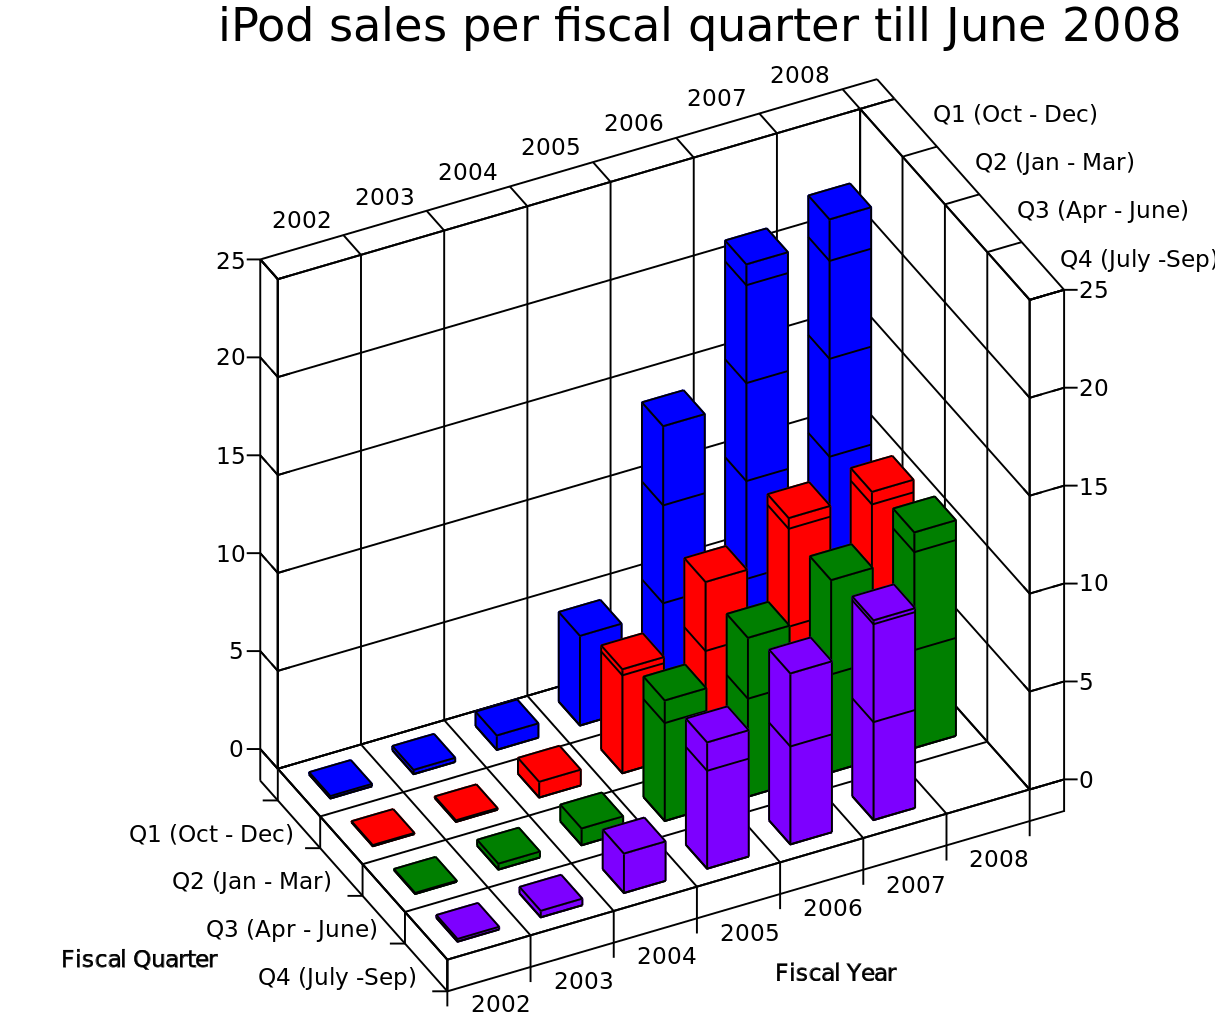
\includegraphics[height=.8\textheight]{images/ipodsales.png}
\end{center}
\vspace{0.5em}
{\tiny Source: \href{https://commons.wikimedia.org/wiki/File:Ipodsales_2008Q3_3d.svg}{Wikimedia}}
}


\frame{
\begin{center}
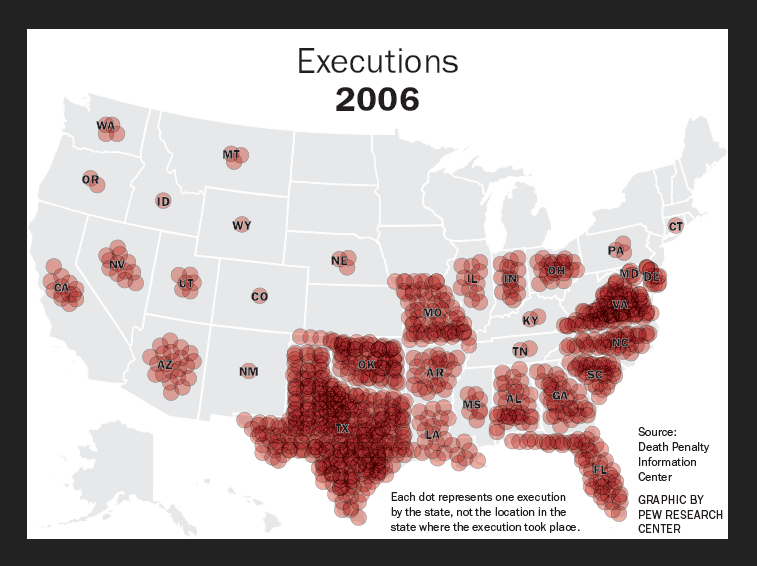
\includegraphics[height=.8\textheight]{images/executions.png}
\end{center}
\vspace{0.5em}
{\tiny Source: \href{http://junkcharts.typepad.com/.a/6a00d8341e992c53ef01a511982206970c-pi}{JunkCharts}}
}

\frame[label=fox1]{
\begin{center}
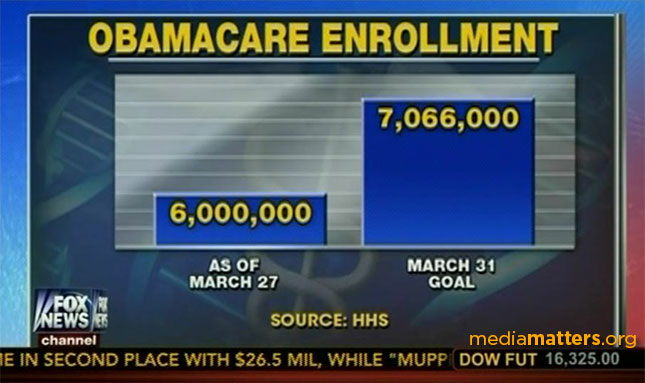
\includegraphics[height=.7\textheight]{images/foxnews1.png}
\end{center}
\vspace{0.5em}
{\tiny Source: \href{http://mediamatters.org/blog/2014/03/31/dishonest-fox-charts-obamacare-enrollment-editi/198679}{MediaMatters}}
}

\frame[label=fox2]{
\begin{center}
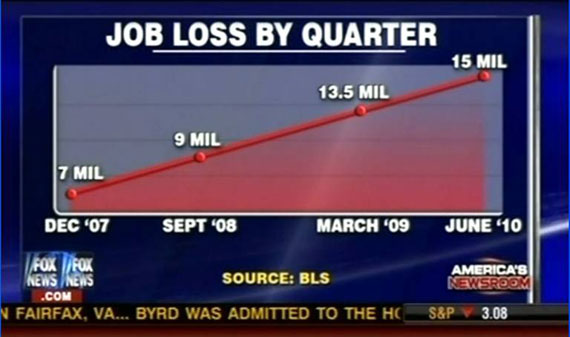
\includegraphics[height=.7\textheight]{images/foxnews2.png}
\end{center}
\vspace{0.5em}
{\tiny Source: \href{http://mediamatters.org/blog/2014/03/31/dishonest-fox-charts-obamacare-enrollment-editi/198679}{MediaMatters}}
}

\frame{
\begin{center}
\only<1>{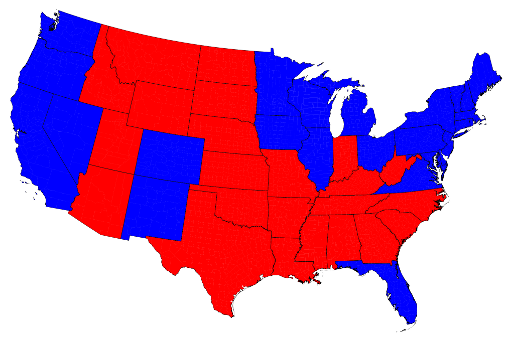
\includegraphics[height=.75\textheight]{images/redblue1.png}}
\only<2>{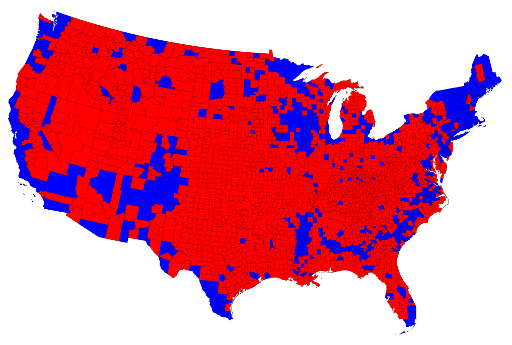
\includegraphics[height=.75\textheight]{images/redblue2.png}}
\only<3>{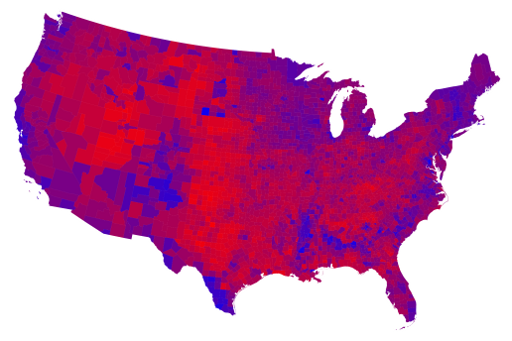
\includegraphics[height=.75\textheight]{images/redblue3.png}}
\only<4>{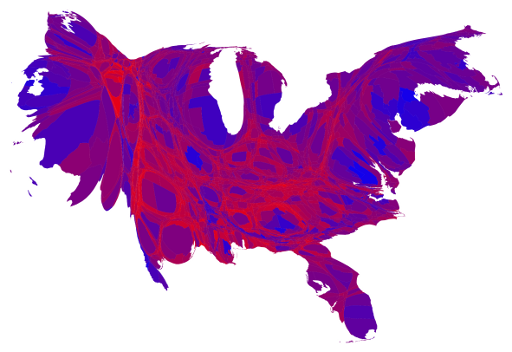
\includegraphics[height=.75\textheight]{images/redblue4.png}}
\end{center}
\vspace{0.25em}
{\tiny Source: \href{http://www-personal.umich.edu/~mejn/election/2012/}{(c) Mark Newman}}
}


\frame{
\frametitle{Visualizations}
\begin{itemize}
\item Definition: ``Data graphics visually display measured quantities by means of the combined use of points, lines, a coordinate system, numbers, symbols, words, shading, and color.'' (Tufte, 2001)
\end{itemize}

\vspace{1em}
{\footnotesize Tufte, E. 2001. \textit{The Visual Display of Quantitative Information}. Graphics Press.}
}



\frame{
\frametitle{Anscombe's Quartet}

{\tiny
\begin{tabular}{rr rr rr rr}
\multicolumn{2}{c}{I} & 
\multicolumn{2}{c}{II} & 
\multicolumn{2}{c}{III} & 
\multicolumn{2}{c}{IV}\\
10.0&8.04&10.0&9.14&10.0&7.46&8.0&6.58\\
8.0&6.95&8.0&8.14&8.0&6.77&8.0&5.76\\
13.0&7.58&13.0&8.74&13.0&12.74&8.0&7.71\\
9.0&8.81&9.0&8.77&9.0&7.11&8.0&8.84\\
11.0&8.33&11.0&9.26&11.0&7.81&8.0&8.47\\
14.0&9.96&14.0&8.10&14.0&8.84&8.0&7.04\\
6.0&7.24&6.0&6.13&6.0&6.08&8.0&5.25\\
4.0&4.26&4.0&3.10&4.0&5.39&19.0&12.50\\
12.0&10.84&12.0&9.13&12.0&8.15&8.0&5.56\\
7.0&4.82&7.0&7.26&7.0&6.42&8.0&7.91\\
5.0&5.68&5.0&4.74&5.0&5.73&8.0&6.89\\
\end{tabular}
}

\vspace{0.5em}

$\bar{x}=9$, $Var(x)=11$,\\
$\bar{y} = 7.5$, $Var(y)=4.12$,\\
$Corr(x,y) = 08.16$
}

\frame{
\frametitle{Anscombe's Quartet}
\begin{center}
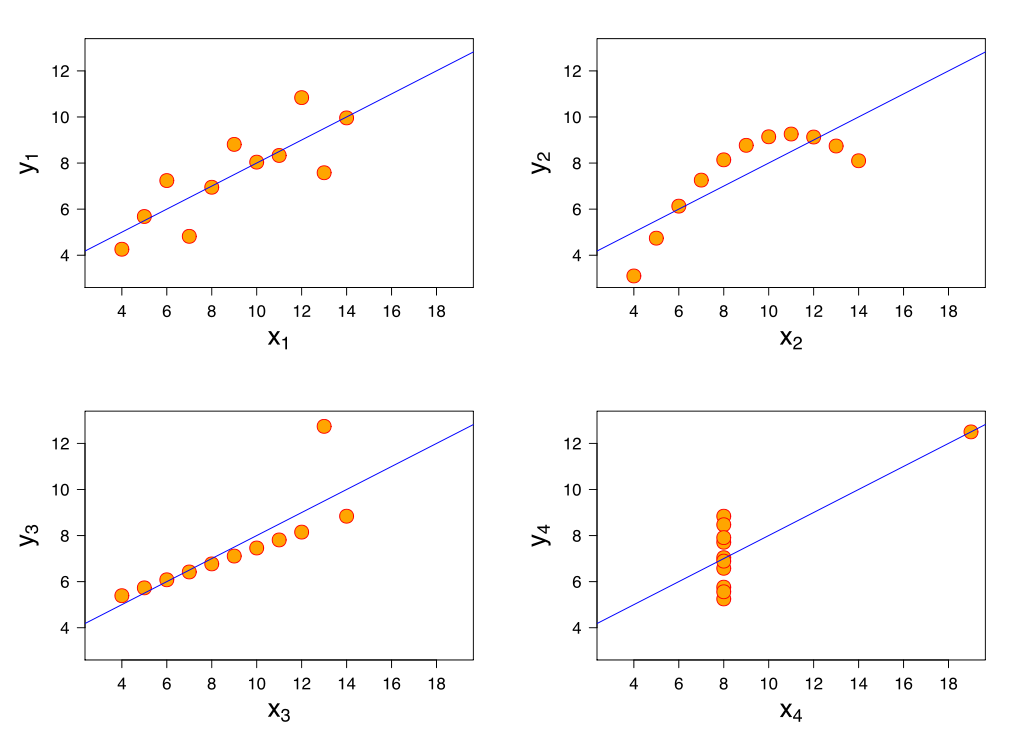
\includegraphics[height=.7\textheight]{images/anscombe.png}
\end{center}
\vspace{0.5em}
{\tiny Source: \href{https://commons.wikimedia.org/wiki/File:Anscombe\%27s_quartet_3.svg}{Wikimedia}}
}


\frame{
\frametitle{{\normalsize Simpson's Paradox}}
\begin{center}
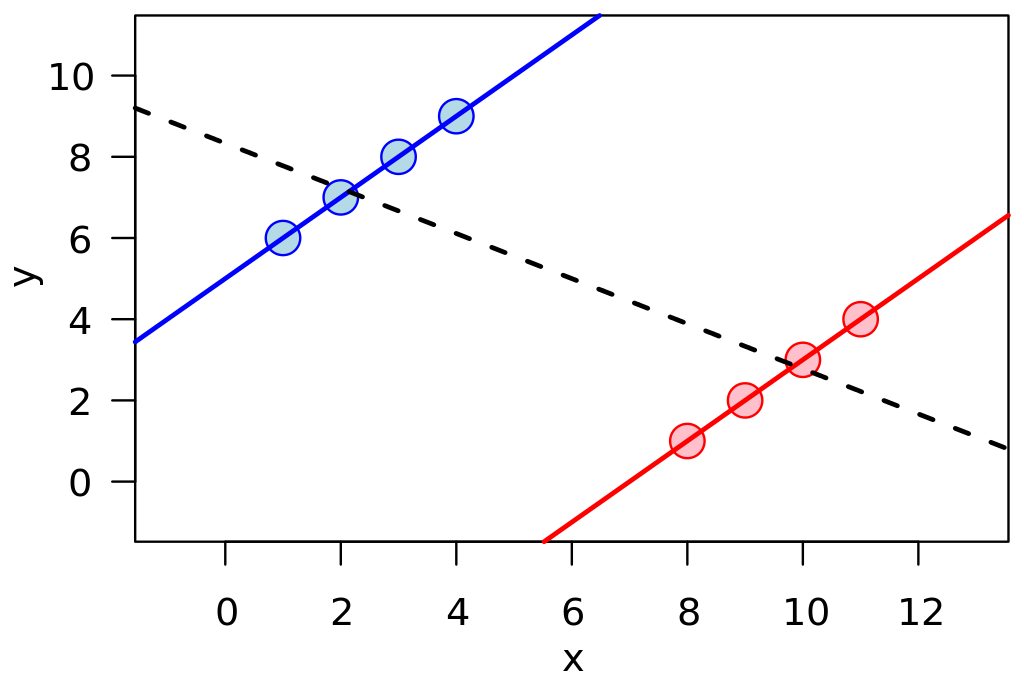
\includegraphics[height=.65\textheight]{images/simpsons.png}
\end{center}
\vspace{0.5em}
{\tiny Source: \href{https://commons.wikimedia.org/wiki/File:Simpson\%27s_paradox_continuous.svg}{Wikimedia}}
}


\frame{
\frametitle{{\normalsize William Playfair}}
\begin{center}
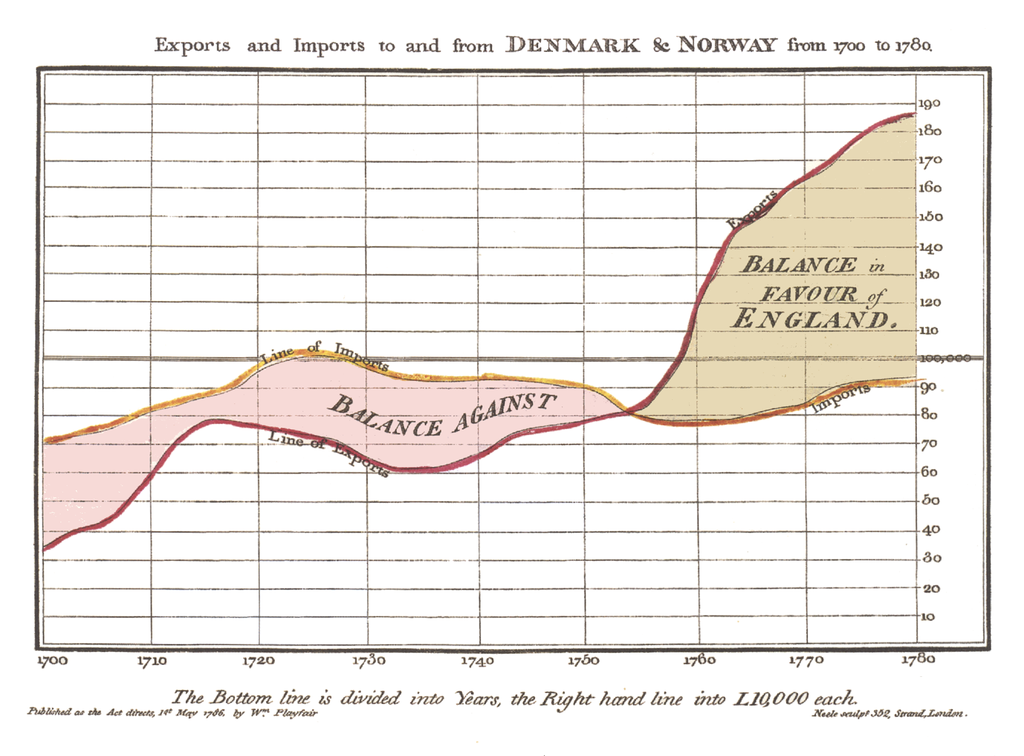
\includegraphics[width=\textwidth]{images/playfair.png}
\end{center}
{\tiny Source: \href{https://commons.wikimedia.org/wiki/File:Minard.png}{Wikimedia}}
}


\frame{
\frametitle{{\normalsize Charles Minard}}
\begin{center}
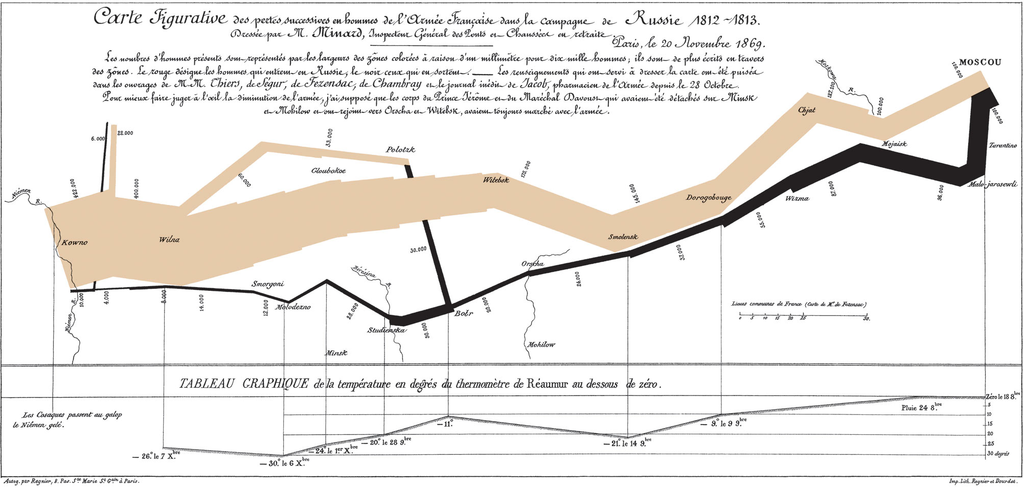
\includegraphics[width=1.05\textwidth]{images/minard.png}
\end{center}
{\tiny Source: \href{https://commons.wikimedia.org/wiki/File:Playfair_TimeSeries-2.png}{Wikimedia}}
}

\frame{
\frametitle{{\normalsize Florence Nightingale}}
\begin{center}
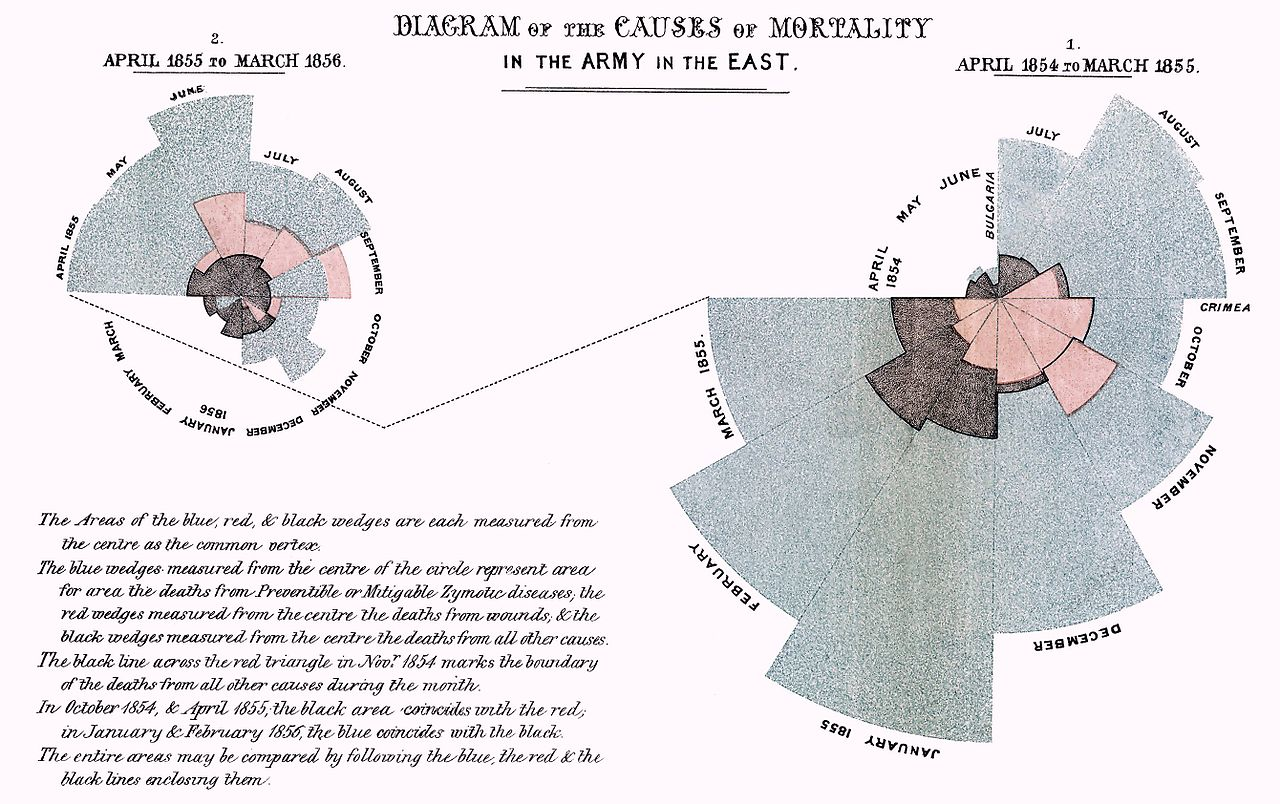
\includegraphics[height=.7\textheight]{images/rose.png}
\end{center}
\vspace{-0.5em}
{\tiny Source: \href{https://commons.wikimedia.org/wiki/File:Nightingale-mortality.jpg}{Wikimedia}}
}





% Do graphs address confounding?





\frame<1>[label=principles]{

\frametitle{Some Basic Principles}
\begin{enumerate}
\item<1-> Be honest
\item<2-> Data-Ink Ratio
\item<3-> Tell a story
\item<4-> Steer reader's attention
\item<5-> Use balanced colour palettes
\end{enumerate}

}

\againframe{fox1}

\againframe{fox2}


\frame{
\begin{center}
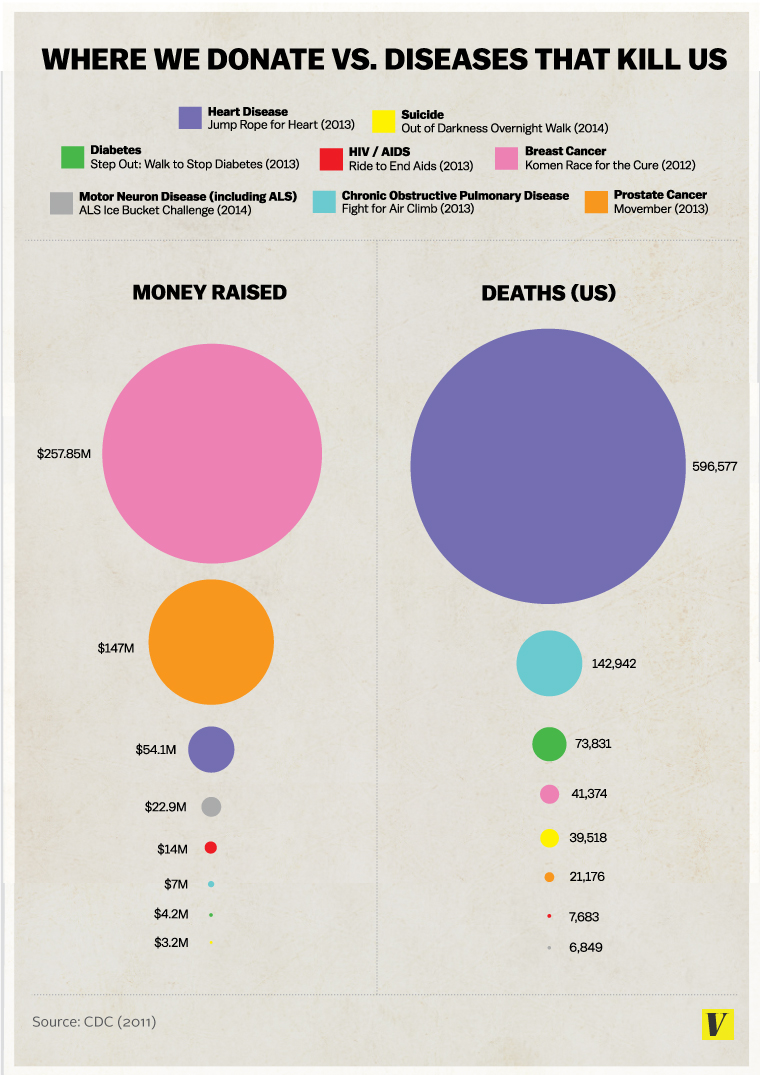
\includegraphics[trim=0in 4in 0in 0in, clip,height=\textheight]{images/vox1.png}
\end{center}

{\footnotesize Source: \href{http://t.co/UjR9o1MjBW}{Vox.com}}
}

\frame{
\begin{center}
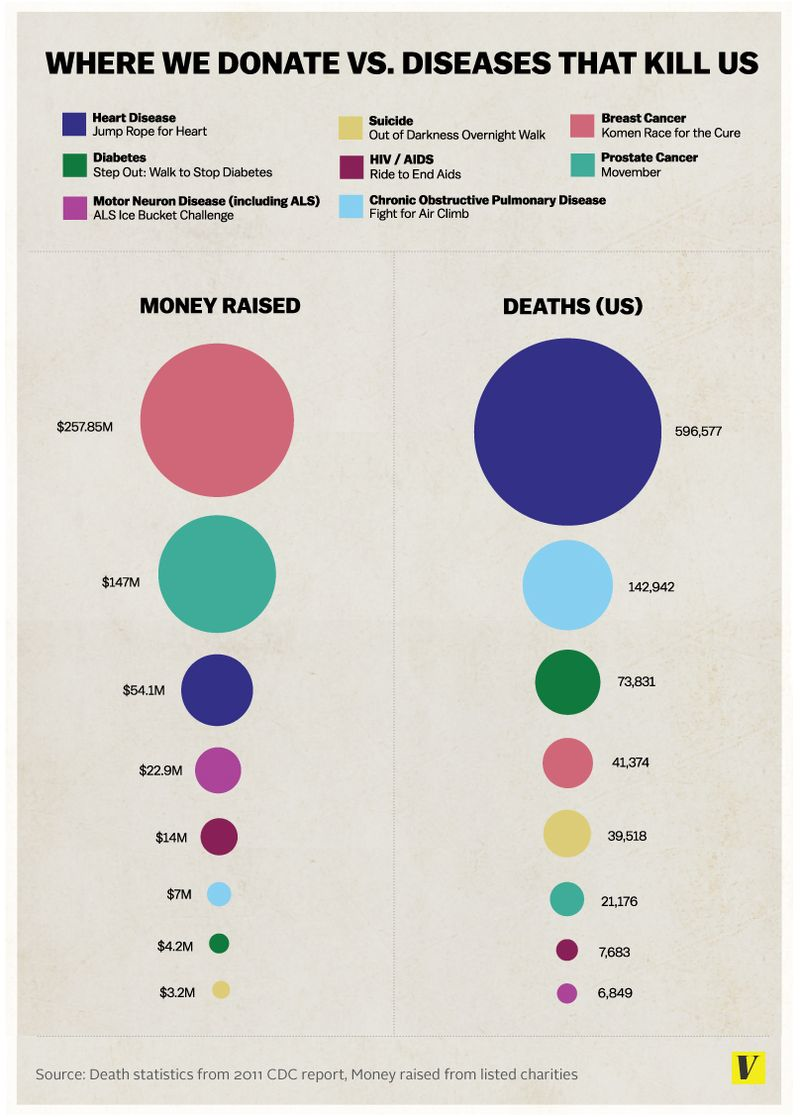
\includegraphics[trim=0in 4in 0in 0in, clip,height=\textheight]{images/vox2.png}
\end{center}

{\footnotesize Source: \href{http://t.co/UjR9o1MjBW}{Vox.com}}
}


\againframe<1-2>{principles}

\frame{
\begin{center}
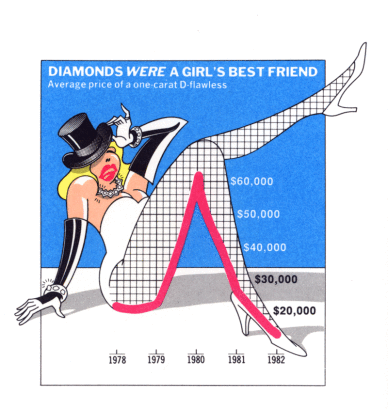
\includegraphics[height=\textheight]{images/tuftediamonds1.png}
\end{center}
}

\frame{
\begin{center}
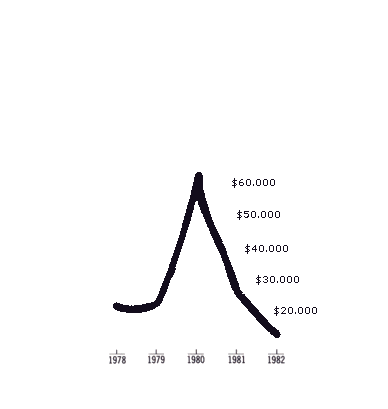
\includegraphics[height=\textheight]{images/tuftediamonds2.png}
\end{center}
}

\frame{
\begin{center}
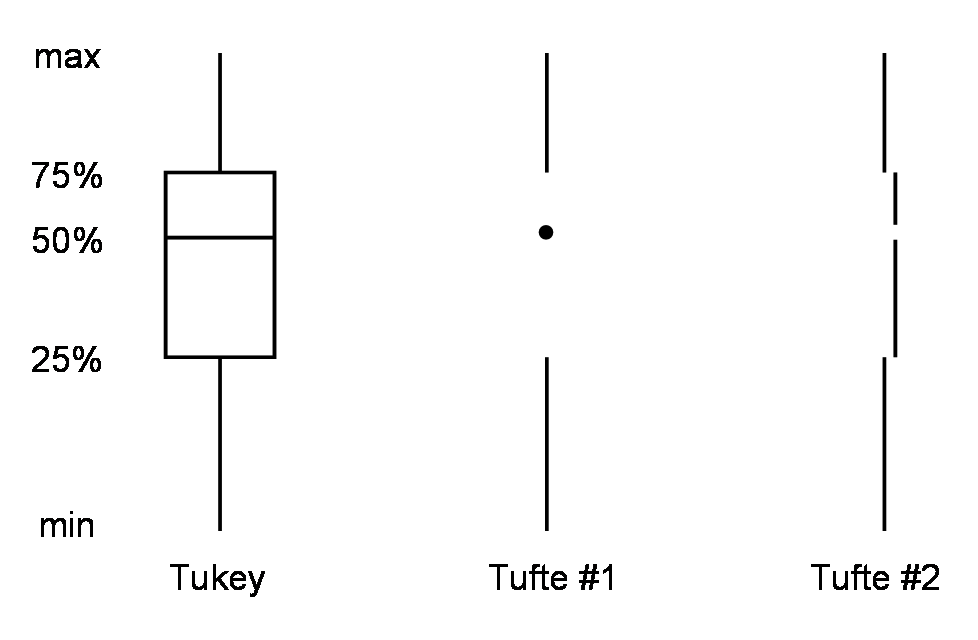
\includegraphics[width=\textwidth]{images/tufteboxplot.png}
\end{center}

{\footnotesize Source: \href{http://stackoverflow.com/questions/24152177/controlling-spacing-in-custom-ggplot2-geoms}{StackOverflow}}
}



\againframe<2-3>{principles}


\frame{
\begin{center}
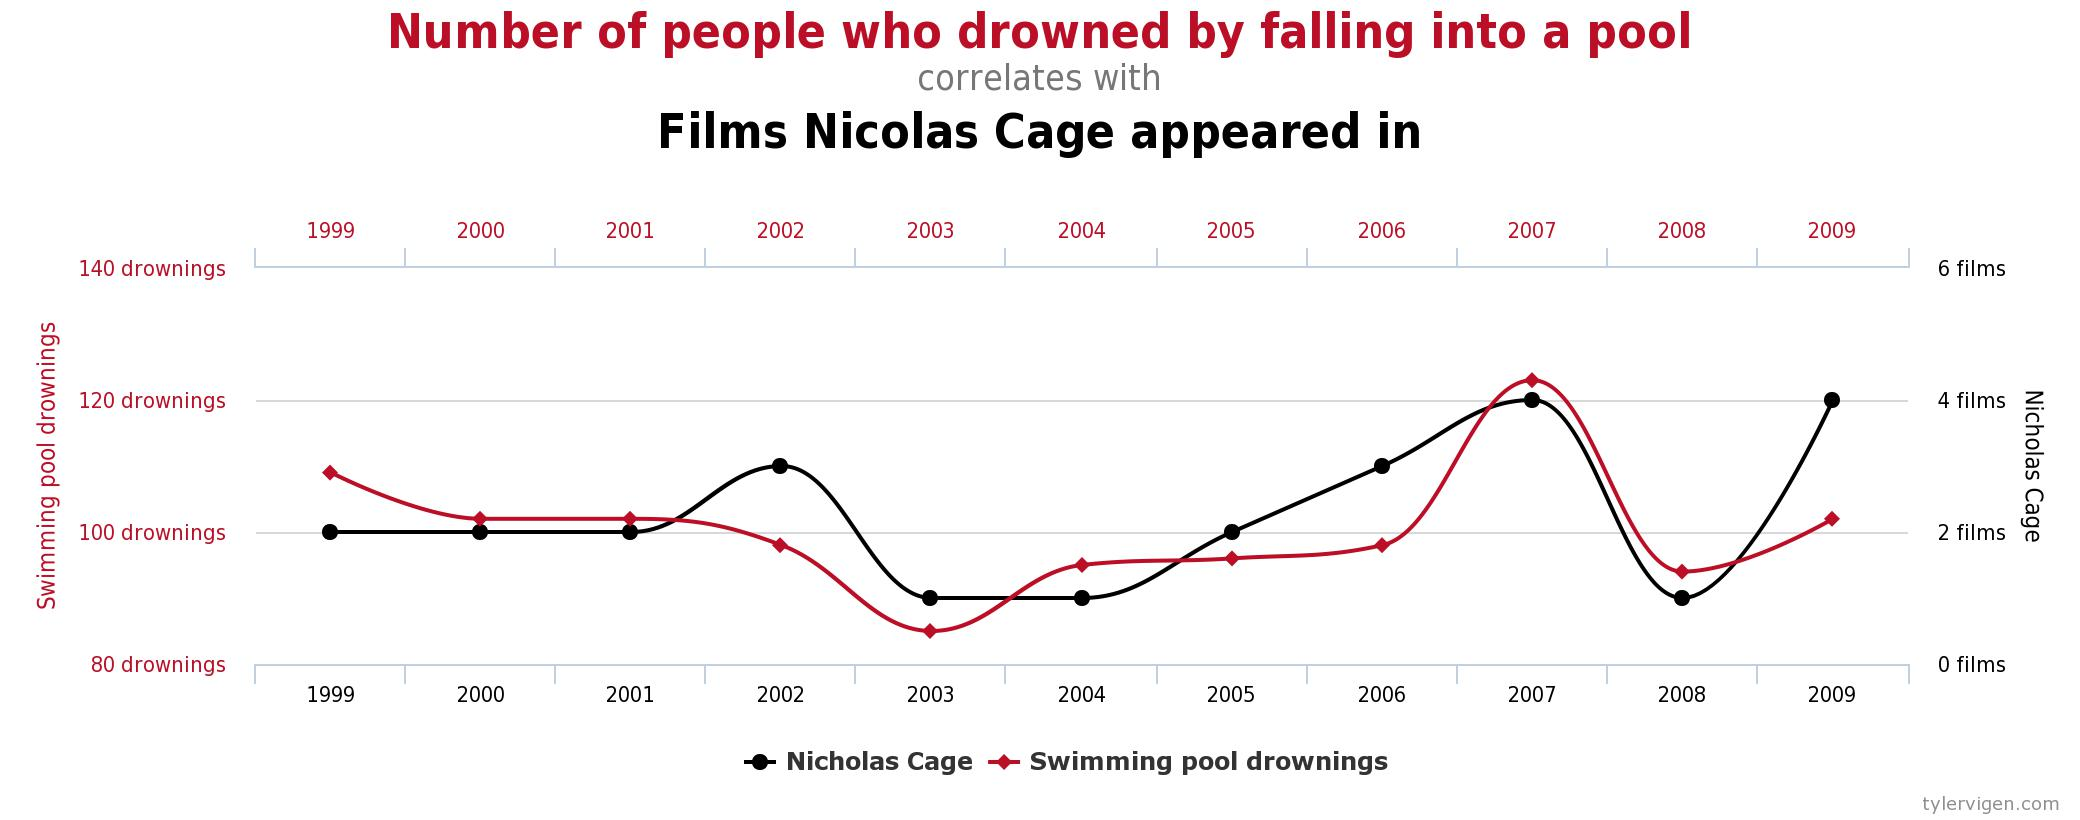
\includegraphics[width=\textwidth]{images/nicholascage.png}
\end{center}
\vspace{-0.5em}
{\tiny Source: \href{http://www.tylervigen.com/about}{CC-BY Tyler Vigen}}
}


\againframe<3-4>{principles}

\frame{
\begin{center}
\only<1>{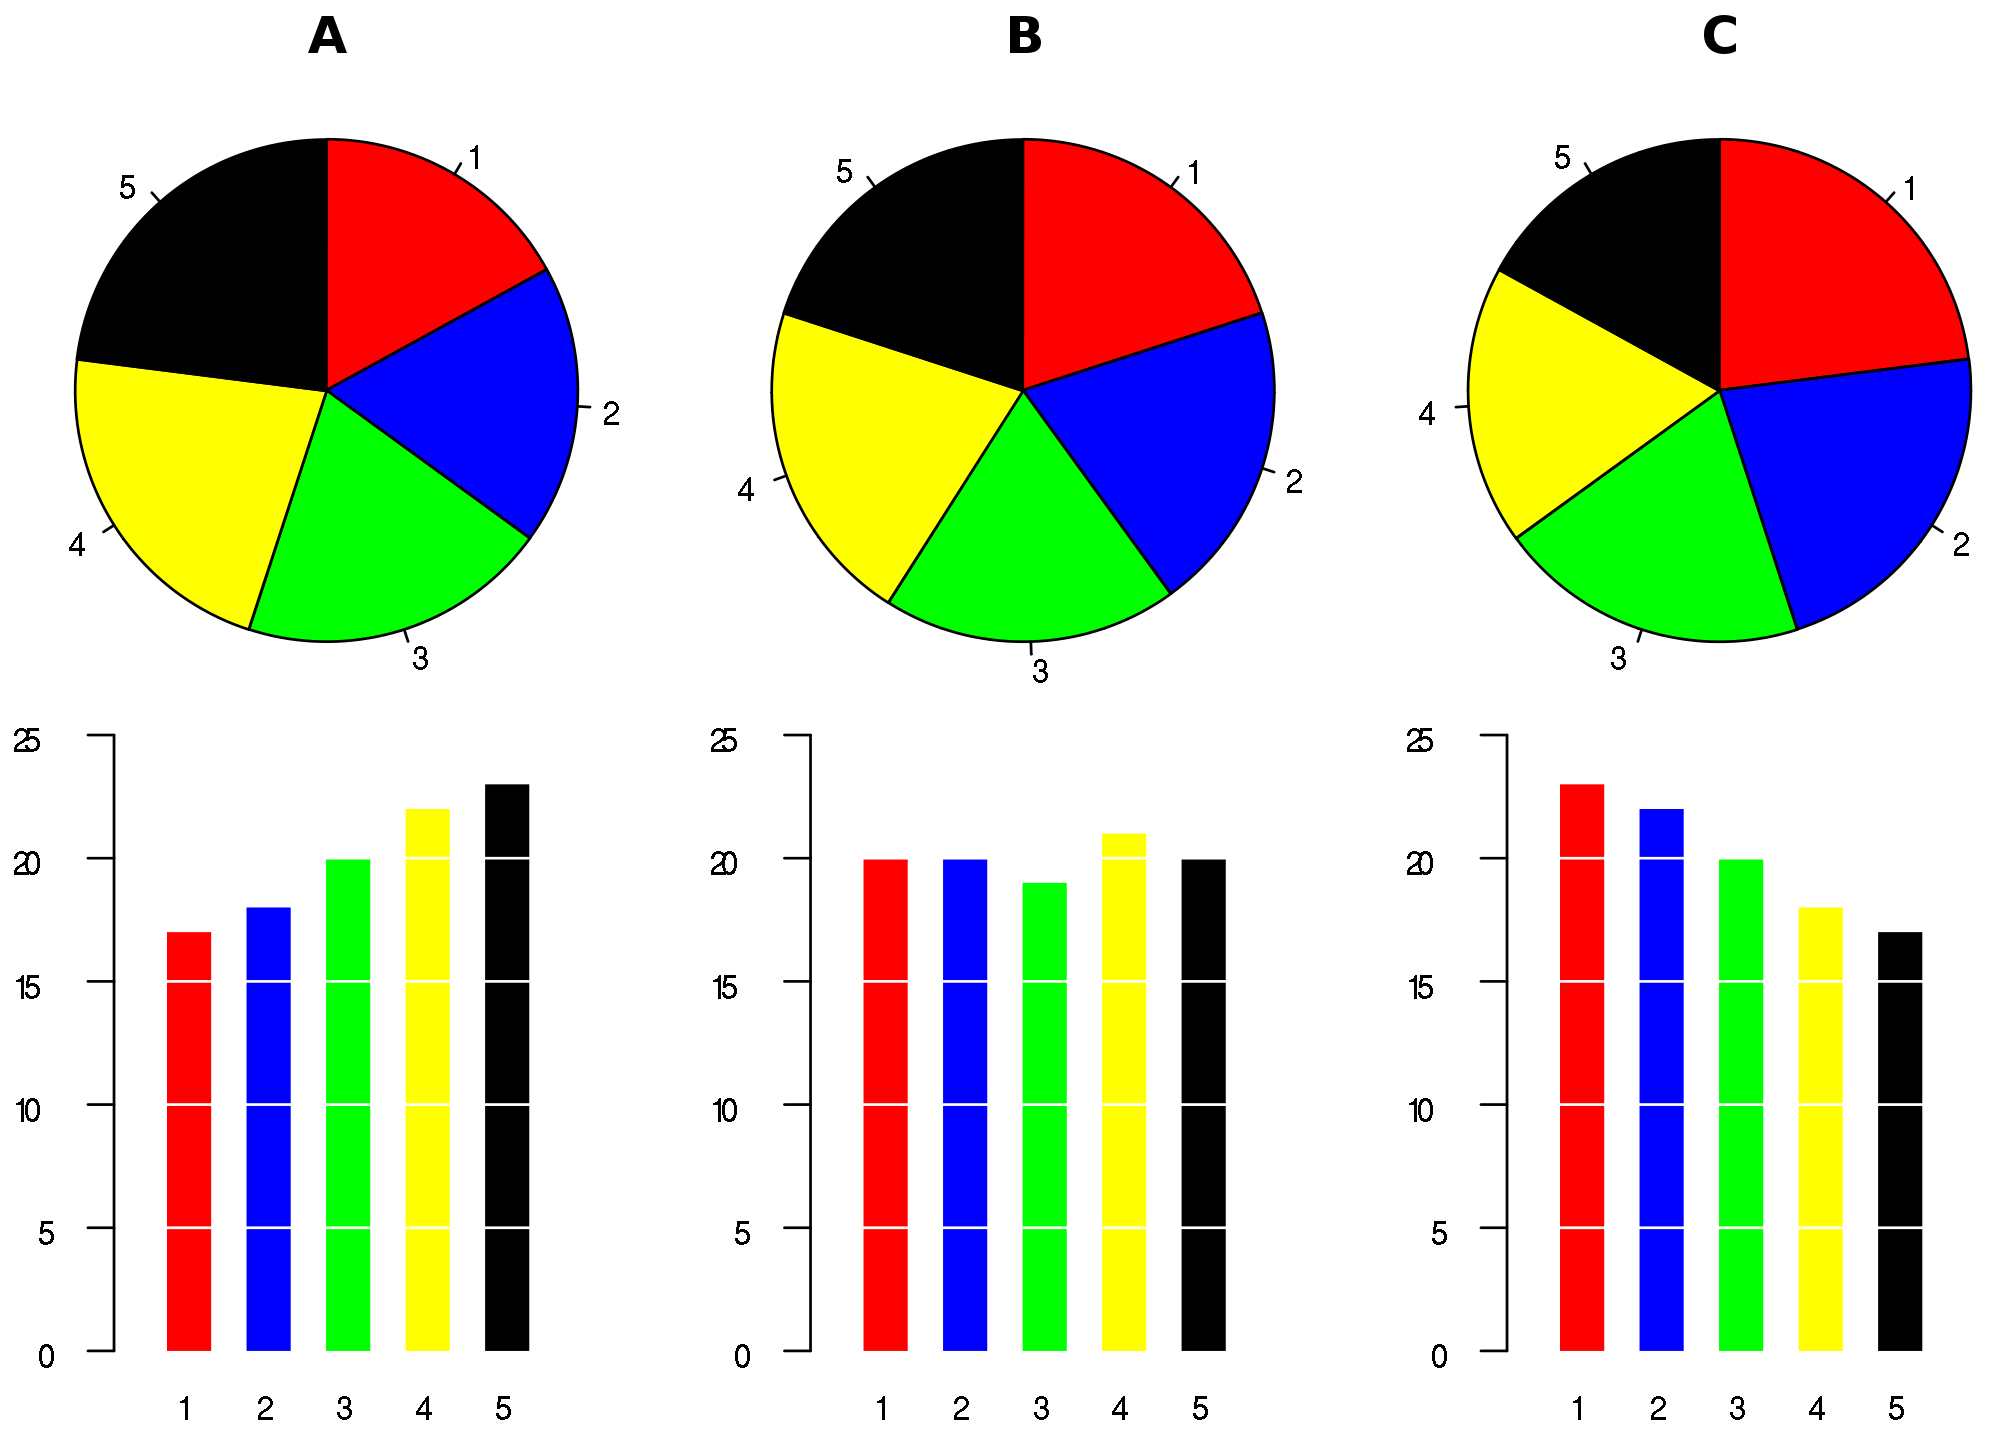
\includegraphics[trim=0in 10in 0in 0in, clip, width=\textwidth]{images/piechart.png}}
\only<2>{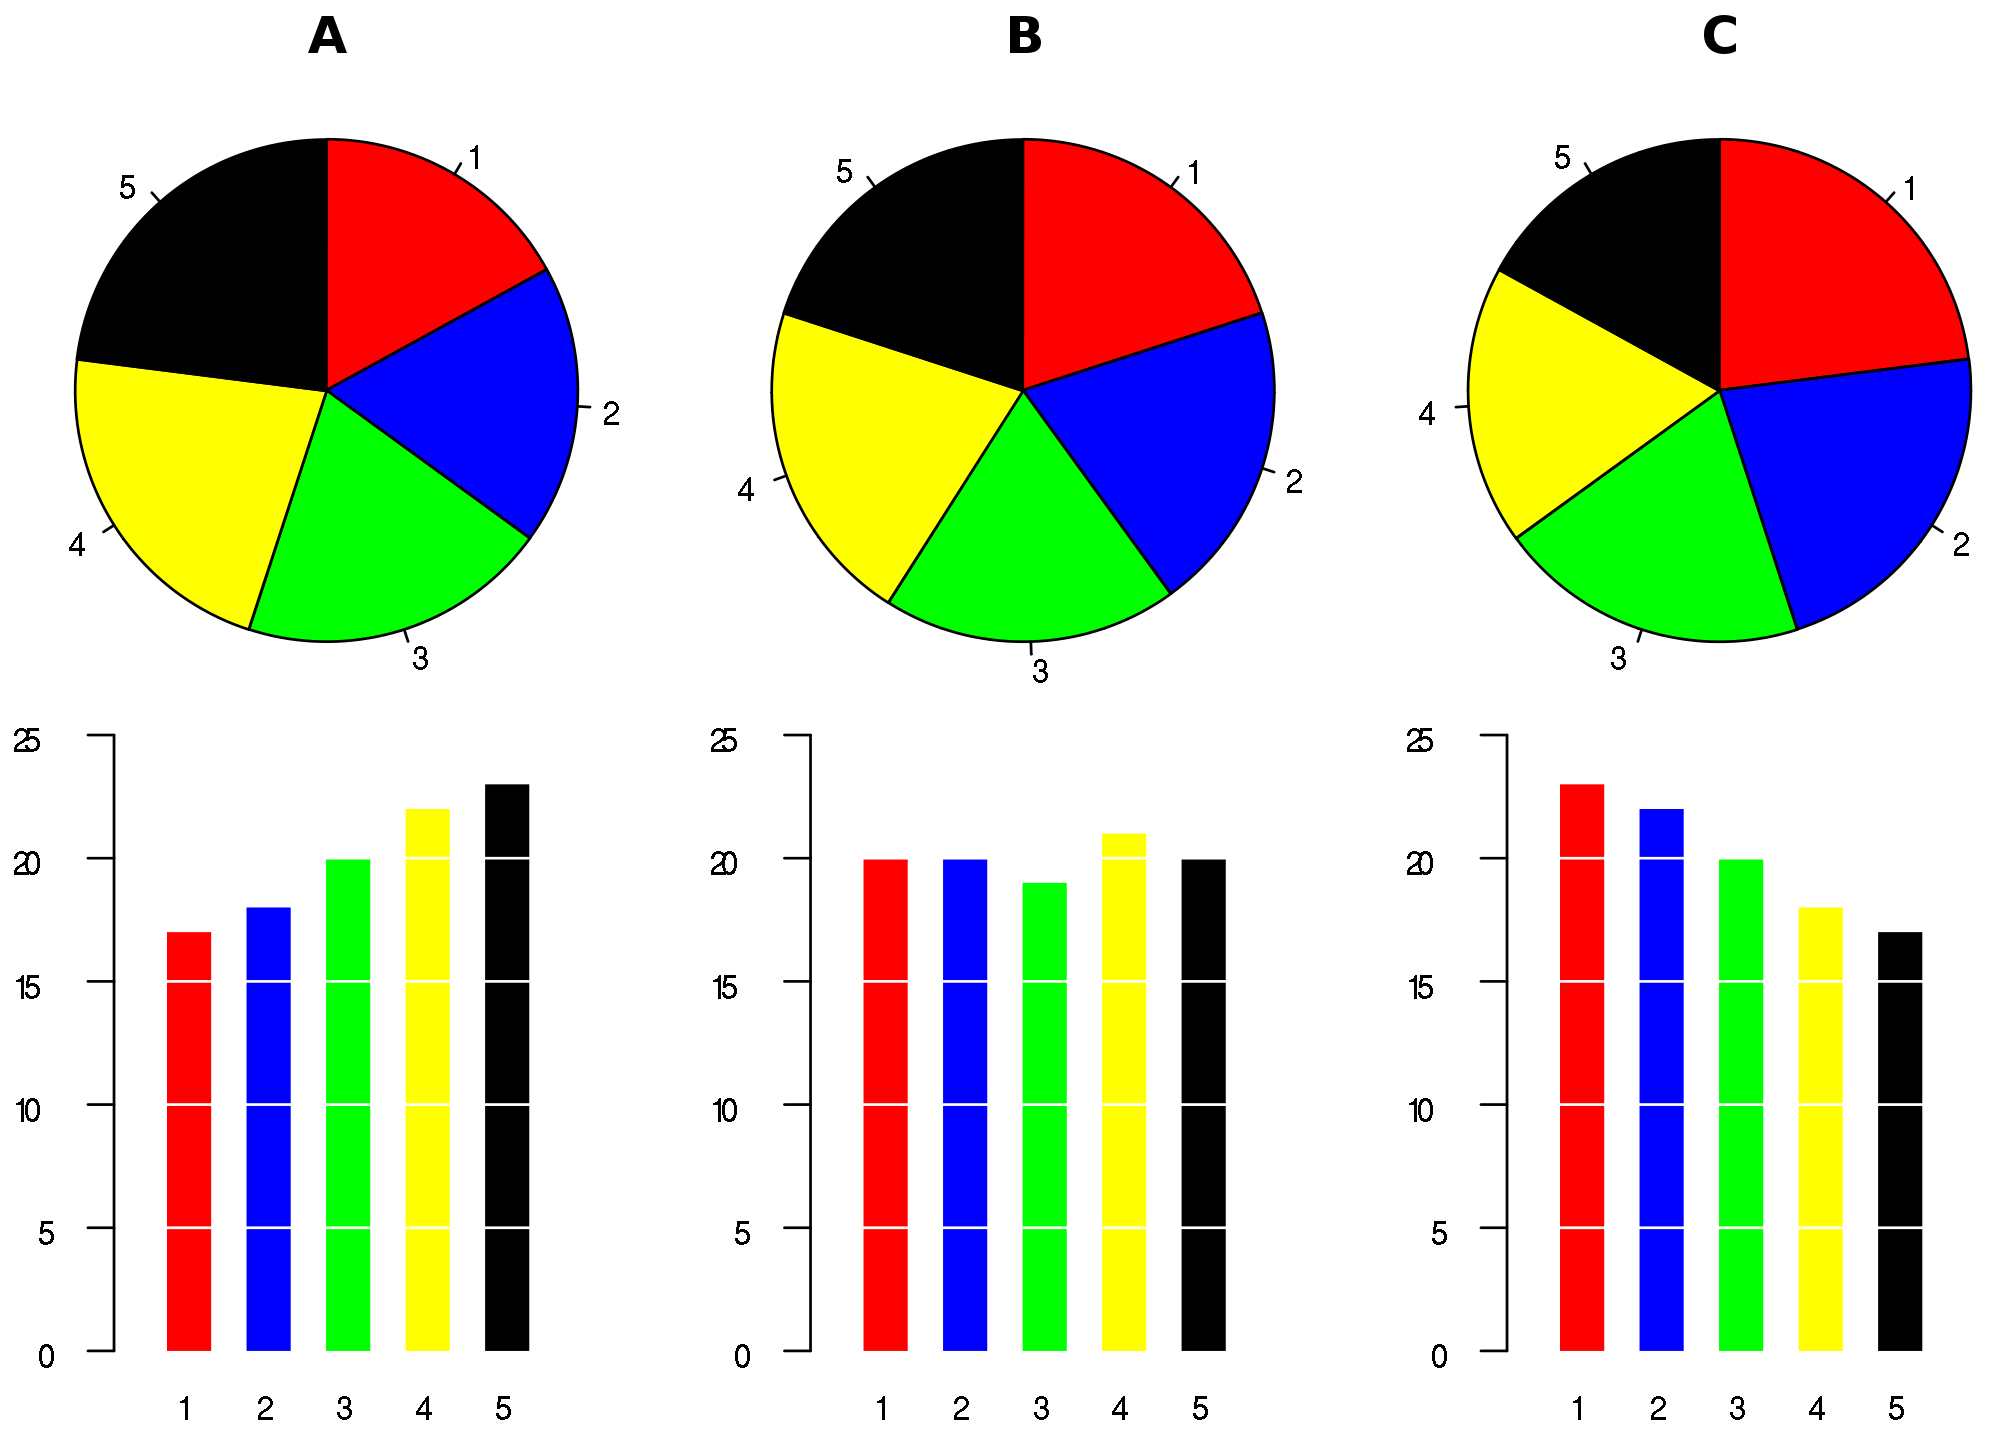
\includegraphics[width=\textwidth]{images/piechart.png}}
\end{center}
\vspace{-0.5em}
{\tiny Source: \href{https://commons.wikimedia.org/wiki/File:Piecharts.svg}{Wikimedia}}
}



\againframe<4-5>{principles}

\frame{
\begin{center}
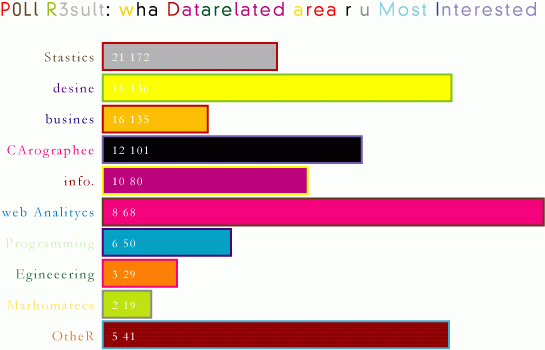
\includegraphics[width=\textwidth]{images/flowingdata.png}
\end{center}
\vspace{-0.5em}
{\tiny Source: \href{https://flowingdata.com/2009/06/15/6-easy-steps-to-make-your-graph-really-ugly/}{Flowing Data}}
}



\frame{
\begin{center}
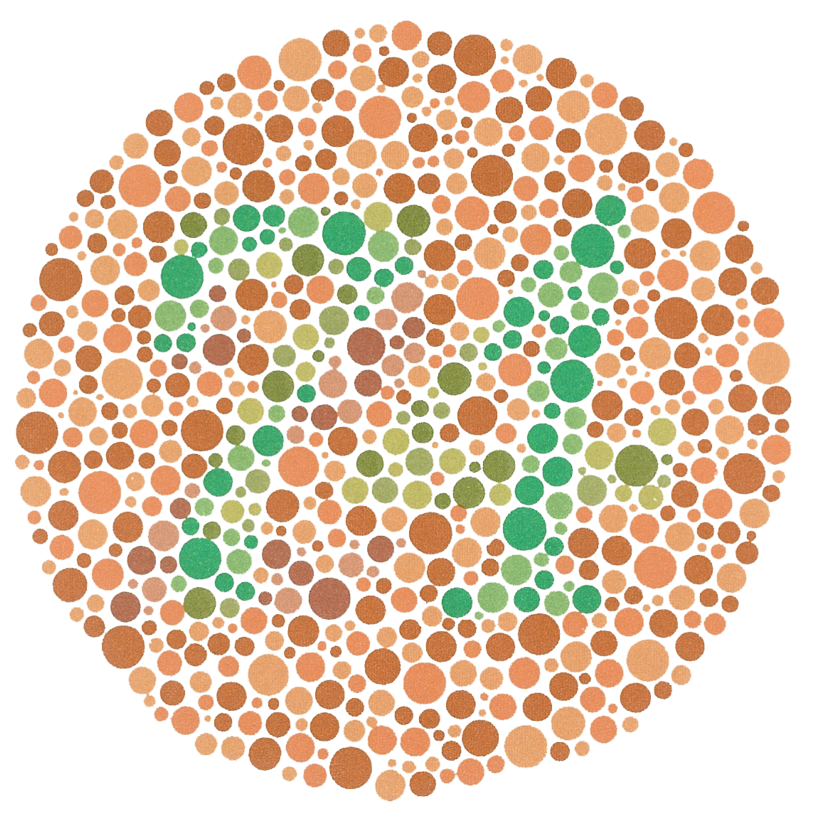
\includegraphics[width=.7\textwidth]{images/colorblindness.png}
\end{center}
\vspace{-1em}
{\tiny Source: \href{https://commons.wikimedia.org/wiki/File:Ishihara_9.png}{Wikimedia}}
}


\frame{
\frametitle{The bottom line}

A visualization should be a display of quantitative (and/or qualitative) data that tells an information-rich story in an honest and beautiful manner.

\vspace{3em}

\onslide<2->{Questions?}

}

\frame{
\frametitle{Homework}

\begin{enumerate}
\item Find a visualization anywhere on the internet.
\item Post a link to the visualization to the Moodle forum.
\item Include the visualization as an image.
\item Describe:
	\begin{itemize}
	\item What is being visualized
	\item Strengths of the visualization
	\item Weaknesses of the visualization
	\end{itemize}

\end{enumerate}


}


\frame{}


\frame{
\frametitle{In R\dots}

R has 5+ graphics ``systems''

\begin{itemize}
\item Base graphics
\item The \textbf{ggplot2} package
\item The \textbf{lattice} package
\item The \textbf{plotrix} package
\item The \textbf{htmlwidgets} package + JavaScript's \href{https://cran.r-project.org/web/packages/plotrix/index.html}{d3 library}
\end{itemize}
}


\frame{
\frametitle{ggplot2}

\begin{itemize}\itemsep1em
\item Most coherent graphics system
\item Based on a ``grammar'' of graphics
\item Easily customized using various ``themes''
	\begin{itemize}
	\item Some built-in to ggplot2
	\item Some in an add-on package (\href{https://cran.r-project.org/web/packages/ggthemes/vignettes/ggthemes.html}{\textbf{ggthemes}})
	\end{itemize}
\end{itemize}
}


\frame{
\frametitle{A bit about the grammar}

\small

\begin{itemize}\itemsep0.25em
\item \texttt{ggplot()} creates a plot object
\item \texttt{aes} describes a mapping of data to a visual element (e.g., color, shape, etc.)
\item \texttt{geom\_*()} displays a particular graphical representation
\item \texttt{scale\_*()} modifies the axes
\item \texttt{coord\_*()} modifies the coordinate system
\item \texttt{theme\_*()} modifies the overall look
\item \texttt{facet\_*()} creates small multiples
\end{itemize}	

}



\frame{
\frametitle{{\normalsize Ways to display a variable}}

\small

In a scatterplot, \texttt{geom\_point()} allows us to display a variable as:
\footnotesize

\begin{itemize}
\item X/Y Axis variable (via \texttt{aes(x=, y=)})
\item Colour (via \texttt{aes(color=)})
\item Alpha (via \texttt{aes(alpha=)})
\item Size (via \texttt{aes(size=)})
\item Shape (via \texttt{aes(shape=)})
\item Facets (via \texttt{facet\_wrap()})
\item Animation (e.g., \url{http://www.gapminder.org/world})
\end{itemize}
}


\frame{}


\appendix

\begin{frame}[fragile]

\tiny

\begin{verbatim}
library("rio")
d <- import("http://www.qogdata.pol.gu.se/data/qog_std_cs_jan17.dta")

summary(d$wef_lifexp) # life expectancy
summary(d$fh_polity2) # Polity scores
summary(d$gle_cgdpc)  # GDP
summary(d$dpi_finter) # executive term limits
summary(d$bti_cr)     # civil rights index

library("ggplot2")
p <- ggplot(d)
p + aes(x = fh_polity2) + geom_density()
p + aes(x = fh_polity2) + geom_histogram()

p + aes(x = bti_cr) + geom_bar()

p + aes(x = gle_cgdpc, y = wef_lifexp) + geom_point() + 
    scale_x_log10() + scale_y_log10()

p + aes(1, fh_polity2) + geom_boxplot()
p + aes(factor(bti_cr), fh_polity2) + geom_boxplot()

p + aes(x = gle_cgdpc, y = wef_lifexp) + geom_point(aes(color = fh_polity2))
p + aes(x = fh_polity2, y = wef_lifexp) + geom_point(aes(size = gle_cgdpc))

p + aes(x = fh_polity2, y = wef_lifexp) + geom_point() + theme_bw()
\end{verbatim}

\end{frame}


\frame{
\frametitle{ggplot2 Resources}

\small
\begin{itemize}
\item \url{http://docs.ggplot2.org/current/}
\item \url{https://www.rstudio.com/wp-content/uploads/2015/03/ggplot2-cheatsheet.pdf}
\item \url{https://github.com/jennybc/ggplot2-tutorial}
\item \url{http://inundata.org/2013/04/10/a-quick-introduction-to-ggplot2/}
\item \url{http://www.cookbook-r.com/Graphs/}
\end{itemize}

}


\frame{
\frametitle{General Resources}

\small

\begin{itemize}
\item \url{http://www.edwardtufte.com/tufte/}
\item \url{http://www.informationisbeautiful.net/}
\item \url{http://flowingdata.com/}
\item \url{http://ourworldindata.org/}
\item \url{http://www.thefunctionalart.com/}
\item \url{http://www.visualisingdata.com/}
\item \url{http://www.braumoeller.info/dataviz/}
\end{itemize}

}

\end{document}
